\chapter{Design And Implemetation Of Embedded Code Service}

Based on the analysis conducted in the previous chapter we now have a clear understanding what Embedded Code Service is, what is its purpose and how it is going to solve outlined problems. In this chapter, we are going to introduce and reason about its design. We are also going to explain what changes need to be done to programming language scanners in order for them to be integrated with Embedded Code Service. At the end of the chapter we will present interesting parts of the implementation based on this design.

\section{Embedded Code Service design}

Firstly, let us summarize the steps that Embedded Code Service has to execute, because it might not be clearly obvious from previous chapters. The goal of the service is to perform data flow analysis of embedded code using one of the already existing scanners to create a data lineage graph of that code which will then be merged with the graph produced by source technology scanner. A programming language scanner works in three steps: extraction of the input, data flow analysis and generating Manta graph. Embedded Code Service needs to perform input orchestration using the provided configuration, then launch all three stages of a scanner and after that help with merging the graphs. The workflow looks as follows (active components are written in parentheses):
\begin{enumerate}
    \item Input orchestration (Embedded Code Service)
    \item Input extraction (scanner's Extractor)
    \item Data flow analysis (scanner's Reader)
    \item Generating lineage graph (Intermediate Dataflow Generator)
    \item Merging graphs (source technology scanner with the help of Embedded Code Service)
\end{enumerate}

\subsection{Multiple programming languages}

The first decision we have to make is whether we want to implement one universal service that can analyze embedded code written in any programming language or whether we want to have specific implementations for each programming language. This decision will greatly influence how the interface of the service is designed. Comparing the two approaches, we chose specific implementations as a more suitable solution.
\par
An initial idea seems to be a universal service, because that is how Dataflow Query Service is implemented. A common service promotes code reuse as multiple parts of the problem will be solved in a similar way regardless of used programming language and data technology, such as merging the graphs of embedded code and source technology. We can also find similarities between the data technologies (e.g., stored procedures written in embedded code in databases) regardless of the programming language used. One service also means that only one component will need to be maintained. The downside of having one service is that its interface needs to be universal, so if one programming language has a different requirement or requires a specific modification, these changes will have to be reflected for other programming languages as well.
\par
One could argue that another benefit of one service is that we have access to the analysis of any embedded code we may find, but that turns out not to be as beneficial as it may sound. In reality, the language of embedded code is always know, so it is easy to use a specific service to analyze it. Having a universal service has been crucial in case of Dataflow Query Service, because it supports recognition of the SQL dialect used in the query, but in case of Embedded Code Service such feature is not needed. When implementing specific services, we can still reach similar code reuse by grouping common logic in base classes, which makes one less argument in favor of a common service. An important advantage that multiple services provide is that they not only allow the interfaces to be tailored to the needs of the programming language scanner, but they also allow different development pace for each service. The fact is that a service for Python is much more preferred by the stakeholders because of its potential and thus a lot more resources are dedicated to working on it. The last argument carries great significance due to its profound impact on the development process, so we decided to implement multiple services, each dedicated for one programming language.
\par
Figure~\ref{fig:ECSbasedesign} shows how a specific service processes embedded code as well as components that is utilizes. The diagram is generic for any programming language.

\begin{figure}[ht]\centering
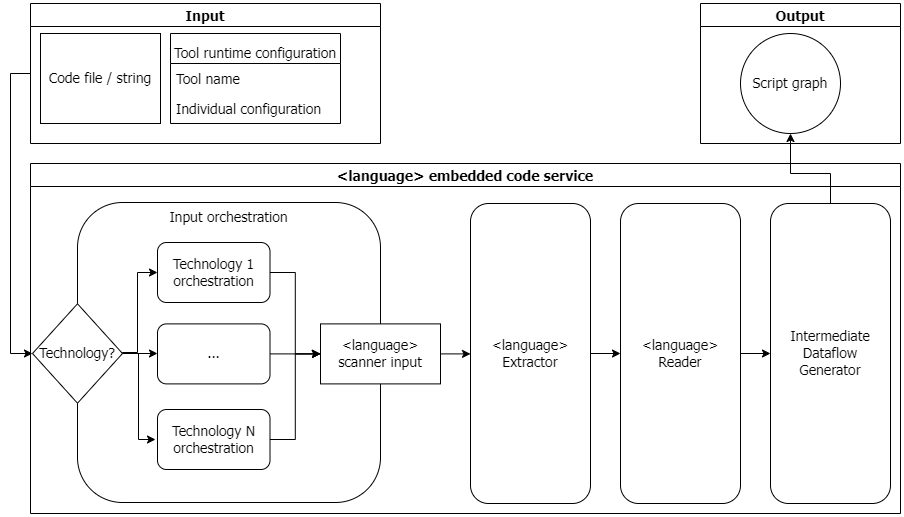
\includegraphics[width=1.0\textwidth]{img/Embedded code service base design.png}
\caption{Diagram of Embedded Code Service workflow}
\label{fig:ECSbasedesign}
\end{figure}   

\subsection{Orchestration}

All contemporary programming languages use some form of import mechanism where the developers can import additional libraries and frameworks. We can see that in embedded code too, often there is a mechanism of adding external libraries to be imported and used by the code. For example in AWS Glue it is possible to define a job argument with a path of Amazon S3 object which contains a custom Python library. When AWS Glue executes a Python job, firstly it checks the S3 location and when it conforms to the required format, it copies the files to the internal working directory next to the job script. When a job is started, Python's import mechanism is able to find these additional libraries and successfully use them in the job script.
\par
Additionally, some technologies (e.g. SAS, Databricks) perform additional orchestration to run the embedded code correctly, such as injecting it in a well-defined class, so this envelope does not have to be written by the user every time, adding the desired imports and only then the embedded code is run on the execution engine used by that technology. This process has to be mimicked by Embedded Code Service before analyzing the code by the scanner to provide an equivalent of the actual code that is executed.
\par
The orchestration process would generally be different for each technology and programming language, but there are some common steps and some repeating patterns. This needs to be reflected in the design of orchestration so the part that needs to be implemented anew when support for new source technology is added is clearly distinguished from common parts. We can use \textit{template method} design pattern, which implements common parts of the process in the base class and lets subclasses redefine certain parts of it. That way we clearly define what can and needs to be implemented.

\subsection{Result}

When the analysis of embedded code is finished, the service shall return a result to source technology scanner. The result is a graph that needs to be merged with another graph and may contain pin nodes that need to be connected. Rather than returning the unfinished graph, we shall return an object that wraps it and provides an interface for connecting pin nodes and merging. The justification is simple, this graph is not always in a valid state so it should be obstructed from the plain view and modification.
\par




%%-subsection-%% 
\subsection{Running the scanner for the embedded code without Manta Flow hooks}
Similarly to the previous problem, this also involves the interface of programming language scanners. These are currently designed to be started by a Manta Flow scenario, responding to hooks. It is desired to modify this interface to enable starting the scanners from Embedded Code Service. These modifications should not be big (the scanners are already quite well designed), but it is important to keep in mind that they need to be finished before a language scanner can be added to the Embedded Code Service. 






%%----- SECTION -----%% Analysis of Python scanner w.r.t. Embedded Code service
\section{Python scanner analysis}

Since the Python scanner wasn't initially designed for running embedded code, we need to analyze what are the required changes in order to support Embedded Code Service (further referenced to as ECS).

\subsection{Interface and Spring configuration}
Python Scanner is designed to analyze user inputs. The source code is provided by users and its location together with other settings is provided in scenario configuration. ECS also receives the input, but not the rest of the configuration. This configuration is supposed to be built during its runtime in input orchestration phase of processing embedded code (see DEV-24356: Python embedded code service - Python scanner interface modifications
DONE
). 
\par
Upon analyzing the current state of the components it is clear that they were designed as single-purpose components - they are constructed with all functional elements and task configuration they require. Therefore, the lifecycle of such component ends when it finishes its task as new component has to be constructed for a new task. This is feasible for language scanners running from CLI, because each scenario executes each task once. With ECS the expected lifecycle of components is different. The service is constructed once but can be used for multiple tasks (e.g., analysis of multiple scripts that are a part of one ETL pipeline).
\par
There are two ways how we can modify current components to support both approaches efficiently. Either add a factory for a component that stores the functional elements for its construction and allow passing the configuration as a parameter in a factory method which constructs the component. This approach is suitable for components which hold a complex internal state and it would be costly to refactor it to a stateless component. Also, it is a cheap modification, there are no changes in code, only a factory needs to be added and this change needs to be reflected in Spring configuration.
\par
The other approach is to modify the component to become a stateless component and the task configuration can be passed using dependency injection. This approach is suitable for components that have a single entry-point - a single method that is invoked to complete the task. In such cases the internal state can be kept internally during the execution of the method and thrown away at the end. Alternatively, this state can be passed between the invocations of multiple methods of the component using dependency injection.

\subsection{CLI}
We need to consider one more thing. The components were designed to work with CLI and their interface is customized for that purpose. ECS doesn’t need to implement such interface. Often this interface doesn’t provide exactly the functionality we need and performs additional tasks that are not required (e.g., serializing output to disk). It would be useful to decouple implementation of the functional component from the CLI interface so the functional component can be used by both CLI and ECS but it can have its own interface to perform required tasks.

\subsection{Components}
There are three major components: Extractor, Reader and Dataflow Generator. These are the components that need to be instantiated for both CLI scanner and Embedded Code Service. We therefore need to focus on their interfaces in the scope of this task.

\subsubsection{Extractor}
Extractor almost satisfies our conditions. The configuration is passed to Extractor in constructor, but it is not necessarily needed. It contains some file paths that are read-only and need to be available during extraction. This component can be easily refactored using the first approach. For CLI use-case the configuration is already stored in ExtractorTask that stores both configuration and extractor, so no Spring configuration changes are required.

\subsubsection{Reader}
Reader is a highly state-dependent component. It would require some effort to remove all application-specific information. However, the current implementation requires some refactoring as it does more things than it should. Also, Reader is currently one component that implements CLI interface and performs the tasks. To satisfy all our conditions we need to:
\begin{enumerate}
    \item Decouple CLI interface from the Reader implementation
    \item Identify static sub-components of Reader
    \item Identify task-specific sub-components of Reader
\end{enumerate}
After the refactoring, static sub-components are a part of EntryPointAnalyzer component which can perform the analysis of a single entry point. Task-specific sub-components are a part of AnalyzerConfiguration. This configuration is like a small toolbox that the analyzer uses during the analysis and is provided for each entry point analysis. Lastly, PythonReader component is the implementation of CLI interface and internally uses an EntryPointAnalyzer and its own static AnalyzerConfiguration for its task. 
\par
With these modifications, the Spring configuration needs to be split in two parts. One is general configuration that provides initialized reusable EntryPointAnalyzer. The other is CLI specific that prepares the AnalyzerConfiguration and binds it with PythonReader.

\subsubsection{Dataflow Generator}
Dataflow Generator was reworked during this analysis so we’ll reference only the current implementation after the rework. It was much more simplified and its dependencies were reduced which makes it much easier to use in various contexts. Currently it requires program ID at construction time which is only used during dataflow generation, so it can be easily refactored to be supplied at that time instead and therefore become stateless. It also requires CLI interface decoupling.
\par
After the refactoring, a new DataflowGenerator class is the stateless component of Dataflow Generator. To transform a graph it needs ProgramConfiguration which holds only the program ID, but it is convenient to be a class so it can be instantiated as a bean. Lastly, the TransformationTask is now just the implementation of the CLI interface, previously it represented all of these new components.

\subsubsection{Configuration}
The Spring configuration of Intermediate Dataflow Generator is layered into multiple levels to introduce modularity. This modularity is important as there are currently 3 language scanners that utilize the generator and each of them is slightly different. Moreover, with the introduction of Embedded Code Service, there is another use-case with different needs.  This design reduces the amount of beans that it depends on to a bare minimum and avoids the need to define beans that are unused.
\par
Currently, there are two possible configuration compositions. One is for scanners that are not supported in Embedded Code Service and the other for those that are. For that purpose the configuration of common beans is split in two where the base context configuration sets up the core component of Dataflow Generator that can be used by the service and the context sets up the dataflow task bean that is required for CLI integration. These configurations can then be included in platform specific configuration that provides platform-specific beans.

\subsubsection{Composition without Embedded Code Service}
Without Embedded Code Service the situation is simple as there is only one use-case, so only the platform-specific beans need to be provided.
\begin{figure}[ht]\centering
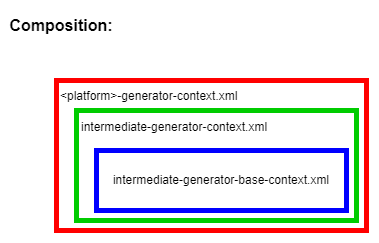
\includegraphics[width=1.0\textwidth]{img/Intermediate Dataflow Generator Configuration-scanner-only composition.png}
\caption{Composition of configurations as they are included in each other}
\label{fig01:ECSbasedesign03}
\end{figure}   
\begin{figure}[ht]\centering
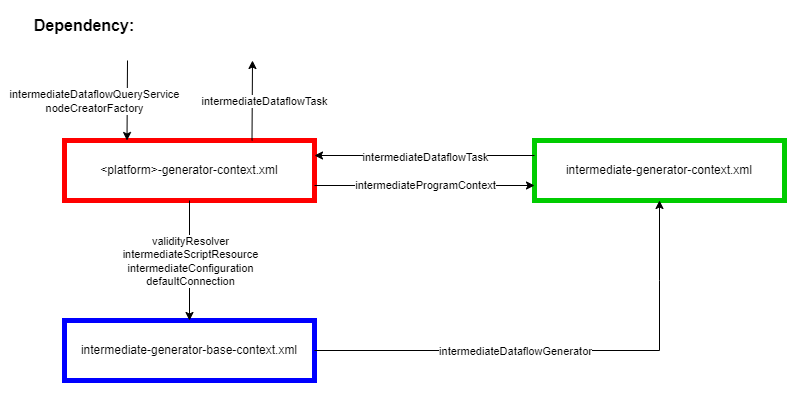
\includegraphics[width=1.0\textwidth]{img/Intermediate Dataflow Generator Configuration-scanner-only dependency.png}
\caption{Dependencies of configurations and their beans}
\label{fig01:ECSbasedesign04}
\end{figure}   

\subsubsection{Composition with Embedded Code Service}
When Embedded Code Service is involved, there needs to be one configuration that satisfies the CLI interfaces and there can be another one that satisfies Code Service needs. Embedded Code Service does not need the CLI interfaces, in fact, they add useless functionality for such use-case, so its best to avoid id. Moreover, in this use-case there could be multiple program configurations passed to Dataflow Generator during its lifecycle so it cannot be defined statically in Spring. To satisfy these needs the platform configurations is split in two parts. First part is configuration of common beans for both use-cases and then there are two specializations that utilize common beans - scanner (CLI) and service specialization.
\begin{figure}[ht]\centering
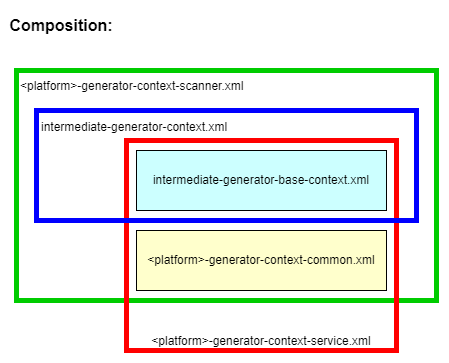
\includegraphics[width=1.0\textwidth]{img/Intermediate Dataflow Generator Configuration-code service-aware composition.png}
\caption{Composition of configurations as they are included in each other}
\label{fig01:ECSbasedesign05}
\end{figure}  
\begin{figure}[ht]\centering
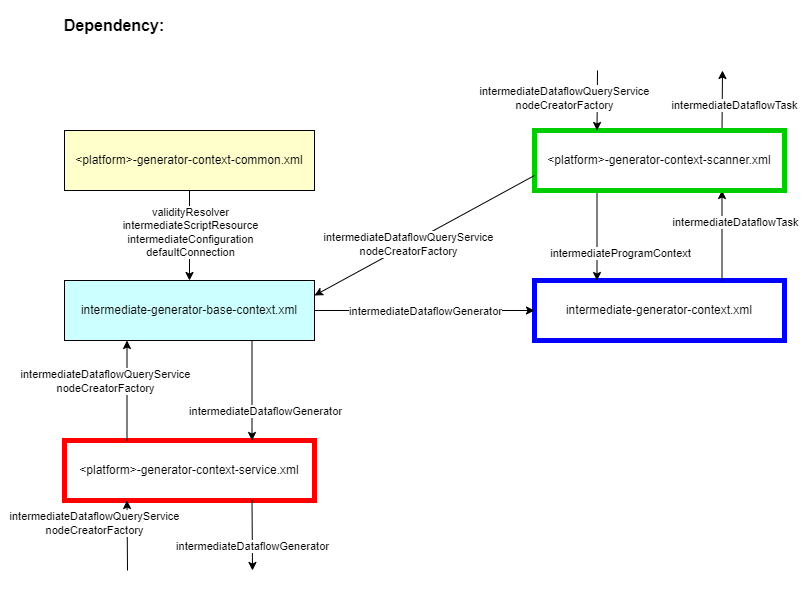
\includegraphics[width=1.0\textwidth]{img/Intermediate Dataflow Generator Configuration-code service-aware dependency.png}
\caption{Dependencies of configurations and their beans}
\label{fig01:ECSbasedesign06}
\end{figure} 




